\subsection{Strahlungsprozesse beschleunigter Elektronen}
\label{subsec:strahlungsprozesse-beschleunigter-elektronen}

Ein Elektron ist nicht nur ein geladenes Teilchen, das auf elektrische und
magnetische Felder reagiert. Wird es beschleunigt oder abgelenkt, so kann es
auch elektromagnetische Strahlung aussenden. Diese Einsicht gehört zu den
zentralen Ergebnissen der klassischen Elektrodynamik.

Der Grundgedanke ist einfach: Eine ruhende Ladung erzeugt ein elektrisches
Feld. Eine gleichförmig bewegte Ladung erzeugt zusätzlich ein magnetisches
Feld. Wird die Ladung jedoch beschleunigt, so ändern sich ihre Felder nicht
nur lokal. Diese Änderung breitet sich als elektromagnetische Welle aus. Das
beschleunigte Elektron kann dabei Energie in Form von Strahlung abgeben.

\begin{PhysicsBox}[Beschleunigte Ladungen strahlen]
	\label{box:beschleunigte-ladungen-strahlen}
	In der klassischen Elektrodynamik gilt:
	Beschleunigte elektrische Ladungen senden elektromagnetische Strahlung aus.
%	\[
%	\text{Beschleunigte elektrische Ladungen senden elektromagnetische Strahlung aus.}
%	\]
	
	Für Elektronen bedeutet das:
	\begin{itemize}
		\item Eine geradlinig beschleunigte oder abgebremste Bewegung kann Strahlung erzeugen.
		\item Eine Ablenkung im Magnetfeld ist ebenfalls eine Beschleunigung, da sich die
		Richtung der Geschwindigkeit ändert.
		\item Die ausgesandte Strahlung trägt Energie vom Elektron weg.
	\end{itemize}
\end{PhysicsBox}

Wichtig ist dabei, dass Beschleunigung nicht nur bedeutet, dass der Betrag der
Geschwindigkeit größer oder kleiner wird. Auch eine reine Richtungsänderung ist
eine Beschleunigung. Ein Elektron auf einer Kreisbahn besitzt daher trotz
konstantem Geschwindigkeitsbetrag eine Zentripetalbeschleunigung. Genau deshalb
können Elektronen auch in Magnetfeldern Strahlung aussenden.

Ein besonders wichtiges Beispiel ist die Bremsstrahlung\index{Bremsstrahlung}.
Sie entsteht, wenn schnelle Elektronen in der Nähe von Atomkernen abgelenkt
oder stark abgebremst werden. Dabei wird ein Teil ihrer Bewegungsenergie in
elektromagnetische Strahlung umgewandelt.
\newpage
\noindent
In einer Röntgenröhre\index{Röntgenröhre} nutzt man genau diesen Effekt:
Elektronen werden durch eine hohe Spannung beschleunigt und treffen anschließend
auf ein Metalltarget. Beim Abbremsen im Material entsteht
Röntgenstrahlung\index{Röntgenstrahlung}.

\begin{PhysicsBox}[Bremsstrahlung]
	\label{box:bremsstrahlung}
	Bremsstrahlung entsteht, wenn schnelle Elektronen durch elektrische Felder,
	vor allem in der Nähe von Atomkernen, stark abgelenkt oder abgebremst werden.
	Dabei verlieren sie Bewegungsenergie, die als elektromagnetische Strahlung
	abgegeben wird.
	
	In einer Röntgenröhre ist dieser Prozess die Grundlage für die Erzeugung von
	Röntgenstrahlung.
\end{PhysicsBox}

Ein zweites wichtiges Beispiel ist die Synchrotronstrahlung\index{Synchrotronstrahlung}.
Sie entsteht, wenn sehr schnelle Elektronen durch Magnetfelder auf gekrümmte
Bahnen gezwungen werden. Obwohl das Magnetfeld selbst keine Arbeit am Elektron
verrichtet, ändert es ständig die Bewegungsrichtung. Diese Richtungsänderung
ist eine Beschleunigung.

Besonders bei sehr hohen, relativistischen Geschwindigkeiten wird die
ausgesandte Strahlung stark und stark nach vorne gebündelt. Synchrotronstrahlung
spielt daher heute eine zentrale Rolle in der Forschung. In großen
Beschleunigeranlagen wird sie genutzt, um Materialien, Moleküle und
Kristallstrukturen mit sehr hoher Genauigkeit zu untersuchen. Zugleich tritt
sie auch in der Astrophysik auf, etwa wenn schnelle Elektronen in kosmischen
Magnetfeldern abgelenkt werden.
\newpage
\noindent
\FloatBarrier
\begin{figure}[H]
	\centering
	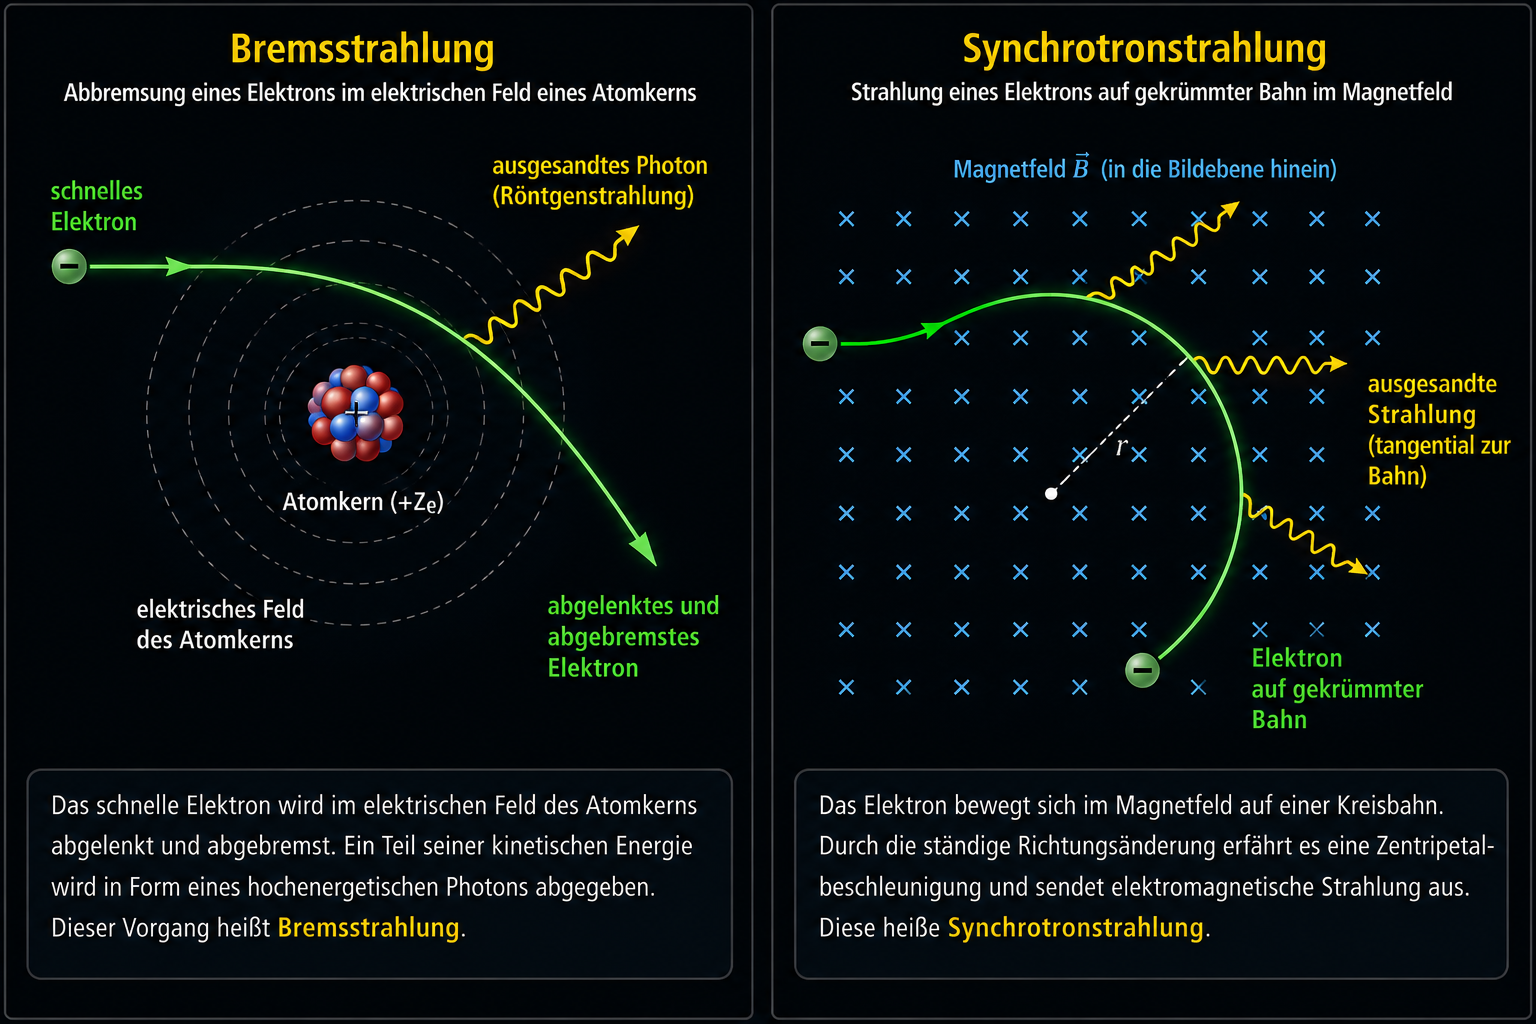
\includegraphics[width=\textwidth]{bilder/bremsstrahlung_synchrotronstrahlung.png}
	\caption{Zwei Strahlungsprozesse beschleunigter Elektronen. Links: Bei der
		Bremsstrahlung wird ein schnelles Elektron in der Nähe eines Atomkerns
		abgelenkt oder abgebremst und gibt dabei elektromagnetische Strahlung ab.
		Rechts: Bei der Synchrotronstrahlung bewegt sich ein Elektron auf einer
		gekrümmten Bahn im Magnetfeld. Durch die ständige Richtungsänderung besitzt
		es eine Beschleunigung und kann Strahlung aussenden.}
	\label{fig:bremsstrahlung-synchrotronstrahlung}
\end{figure}

Die Abbildung~\ref{fig:bremsstrahlung-synchrotronstrahlung} zeigt den
Unterschied der beiden Prozesse: Bei der Bremsstrahlung entsteht die Strahlung
durch das starke Abbremsen oder Ablenken im elektrischen Feld eines Atomkerns.
Bei der Synchrotronstrahlung entsteht sie durch die gekrümmte Bahn eines
Elektrons im Magnetfeld.

Ein wichtiger Punkt darf dabei nicht übersehen werden. In der idealisierten
Betrachtung verrichtet das Magnetfeld keine Arbeit am Elektron, weil die
magnetische Lorentzkraft stets senkrecht zur Geschwindigkeit steht. Der Betrag
der Geschwindigkeit bleibt dann zunächst konstant, und das Magnetfeld ändert
nur die Richtung der Bewegung.
\newpage
\noindent
Sendet das Elektron jedoch Synchrotronstrahlung aus, so trägt diese Strahlung
Energie weg. Ohne äußere Energiezufuhr würde das Elektron daher allmählich
kinetische Energie verlieren. Sein Bahnradius würde kleiner werden, denn für
die Kreisbahn im Magnetfeld gilt

\[
r = \frac{m_e v}{eB}.
\]

Nimmt die Geschwindigkeit \(v\) ab, so nimmt auch der Bahnradius \(r\) ab.
Das Elektron würde also nicht dauerhaft auf derselben Kreisbahn bleiben,
sondern langsam auf eine engere Bahn übergehen. In realen Synchrotronanlagen
wird dieser Energieverlust durch elektrische Beschleunigungsfelder wieder
ausgeglichen. Nur dadurch können die Elektronen über längere Zeit auf einer
stabilen Bahn gehalten werden.

\begin{DidacticBox}[Warum Synchrotronstrahlung Energie kostet]
	\label{box:synchrotronstrahlung-energieverlust}
	Ein Magnetfeld verrichtet keine Arbeit am Elektron. Es ändert nur die Richtung
	der Bewegung, nicht direkt den Betrag der Geschwindigkeit.
	
	Wenn das Elektron jedoch Synchrotronstrahlung aussendet, verliert es Energie.
	Ohne äußere Energiezufuhr würde seine Geschwindigkeit abnehmen und der
	Bahnradius kleiner werden.
	
	In echten Synchrotronanlagen wird dieser Energieverlust durch elektrische
	Beschleunigungsfelder ausgeglichen.
\end{DidacticBox}

Der Zusammenhang zwischen Kreisbewegung und Strahlung zeigt zugleich eine
wichtige Grenze des rein klassischen Elektronenbildes. Nach klassischer
Vorstellung müsste ein Elektron, das im Atom um einen Kern kreist, ständig
Strahlung aussenden und dadurch Energie verlieren. Es würde schließlich in den
Atomkern stürzen. Genau das beobachtet man jedoch nicht: Atome sind stabil.

Diese Schwierigkeit wurde zu einem entscheidenden Hinweis darauf, dass das
Elektron im Atom nicht einfach als klassisches Teilchen auf einer gewöhnlichen
Kreisbahn verstanden werden kann. Die Stabilität der Atome verlangt eine neue
Beschreibung. Sie führt direkt zur Quantenphysik.

\begin{DidacticBox}[Grenze des klassischen Elektronenbildes]
	\label{box:strahlung-und-grenze-klassik}
	Die klassische Elektrodynamik erklärt sehr gut, warum beschleunigte Elektronen
	Strahlung aussenden. Genau dadurch entsteht aber ein Problem:
	
	\begin{itemize}
		\item In Magnetfeldern können Elektronen durch ihre Kreisbewegung strahlen.
		\item In Röntgenröhren entsteht durch Abbremsung Bremsstrahlung.
		\item Im klassischen Atommodell müsste ein kreisendes Elektron ebenfalls
		ständig Strahlung verlieren.
	\end{itemize}
	
	Die Stabilität der Atome zeigt daher: Das klassische Bild des Elektrons ist
	nicht falsch, aber es ist unvollständig.
\end{DidacticBox}

Strahlungsprozesse beschleunigter Elektronen sind damit doppelt wichtig. Sie
erklären einerseits zentrale technische Anwendungen wie Röntgenröhren und
Synchrotronquellen. Andererseits zeigen sie eine tiefe Grenze der klassischen
Physik: Das Verhalten des Elektrons im Atom lässt sich nicht mehr mit
klassischen Bahnen allein verstehen.